\documentclass{standalone}
\usepackage{tikz}
\usetikzlibrary{patterns, positioning}


\begin{document}
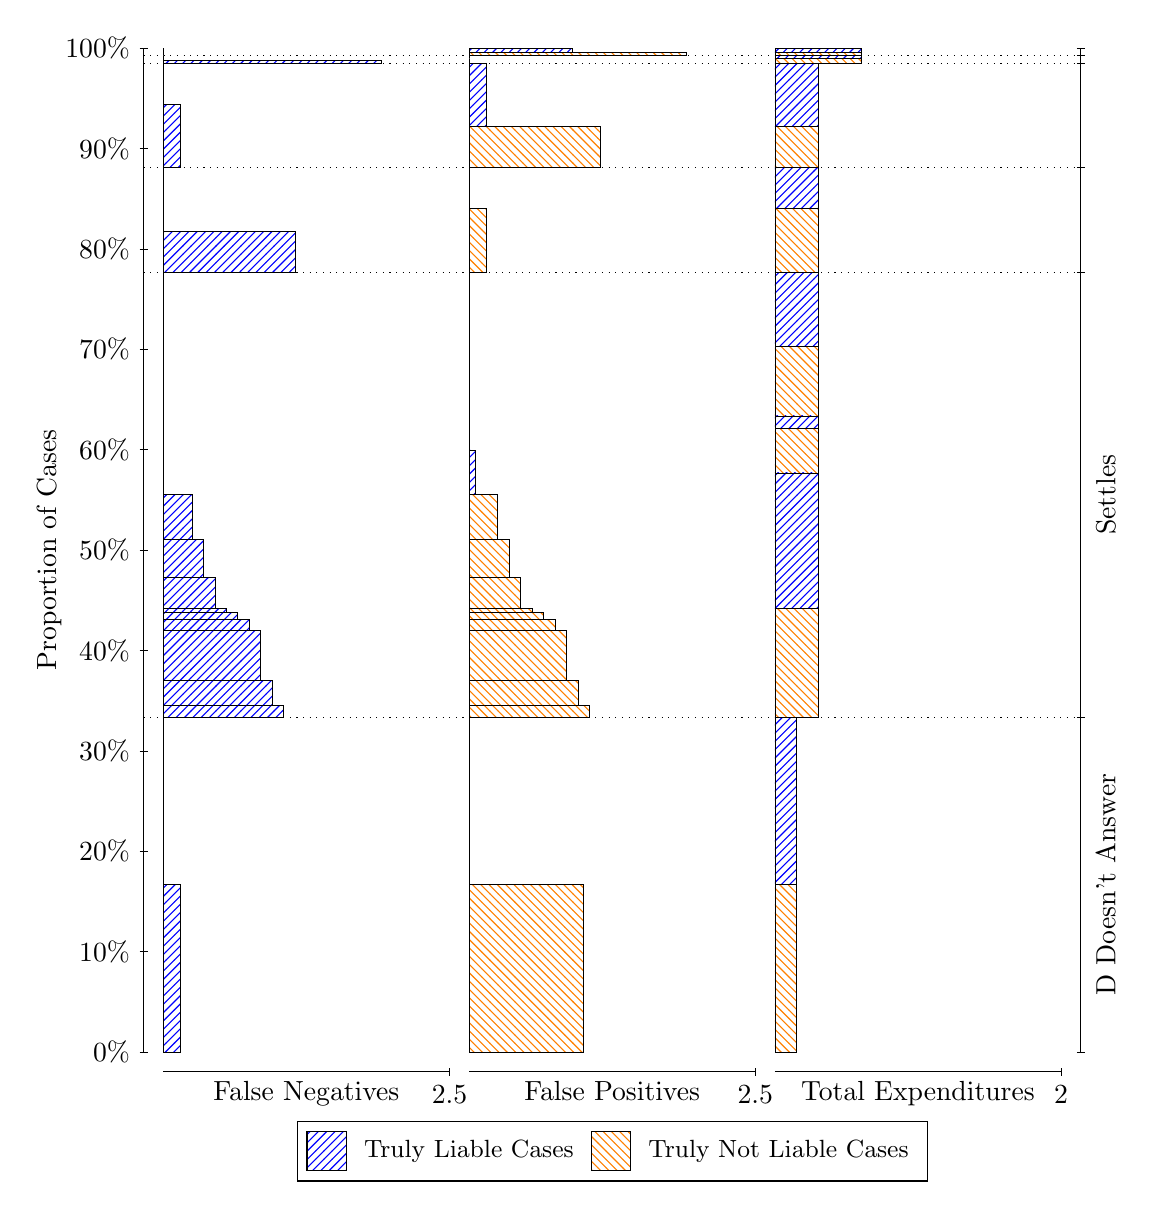
\begin{tikzpicture}
\draw[black, very thin] (1.5,1.75) -- (1.5,14.5);
\node[rotate=90, text=black, anchor=center] at (0.3, 8.125) {Proportion of Cases};
\draw[black, very thin] (1.45,1.75) -- (1.55,1.75);
\node[text=black, anchor=east] at (1.45, 1.75) {0\%};
\draw[black, very thin] (1.45,3.025) -- (1.55,3.025);
\node[text=black, anchor=east] at (1.45, 3.025) {10\%};
\draw[black, very thin] (1.45,4.3) -- (1.55,4.3);
\node[text=black, anchor=east] at (1.45, 4.3) {20\%};
\draw[black, very thin] (1.45,5.575) -- (1.55,5.575);
\node[text=black, anchor=east] at (1.45, 5.575) {30\%};
\draw[black, very thin] (1.45,6.85) -- (1.55,6.85);
\node[text=black, anchor=east] at (1.45, 6.85) {40\%};
\draw[black, very thin] (1.45,8.125) -- (1.55,8.125);
\node[text=black, anchor=east] at (1.45, 8.125) {50\%};
\draw[black, very thin] (1.45,9.4) -- (1.55,9.4);
\node[text=black, anchor=east] at (1.45, 9.4) {60\%};
\draw[black, very thin] (1.45,10.675) -- (1.55,10.675);
\node[text=black, anchor=east] at (1.45, 10.675) {70\%};
\draw[black, very thin] (1.45,11.95) -- (1.55,11.95);
\node[text=black, anchor=east] at (1.45, 11.95) {80\%};
\draw[black, very thin] (1.45,13.225) -- (1.55,13.225);
\node[text=black, anchor=east] at (1.45, 13.225) {90\%};
\draw[black, very thin] (1.45,14.5) -- (1.55,14.5);
\node[text=black, anchor=east] at (1.45, 14.5) {100\%};

\draw[black, very thin] (13.4,1.75) -- (13.4,14.5);
\draw[black, very thin] (13.35,1.75) -- (13.45,1.75);
\node[anchor=west] at (13.35, 1.75) {};
\draw[black, very thin] (13.35,6) -- (13.45,6);
\node[anchor=west] at (13.35, 6) {};
\draw[black, very thin] (13.35,11.653) -- (13.45,11.653);
\node[anchor=west] at (13.35, 11.653) {};
\draw[black, very thin] (13.35,12.98) -- (13.45,12.98);
\node[anchor=west] at (13.35, 12.98) {};
\draw[black, very thin] (13.35,14.307) -- (13.45,14.307);
\node[anchor=west] at (13.35, 14.307) {};
\draw[black, very thin] (13.35,14.404) -- (13.45,14.404);
\node[anchor=west] at (13.35, 14.404) {};
\draw[black, very thin] (13.35,14.5) -- (13.45,14.5);
\node[anchor=west] at (13.35, 14.5) {};

\draw[black, very thin, pattern color=blue, pattern=north east lines] (1.75,1.75) rectangle (1.968,3.875);
\draw[black, very thin, pattern color=orange, pattern=north west lines] (1.75,3.875) rectangle (1.75,6);
\draw[black, very thin, pattern color=blue, pattern=north east lines] (1.75,6) rectangle (3.276,6.156);
\draw[black, very thin, pattern color=blue, pattern=north east lines] (1.75,6.156) rectangle (3.1307,6.4716);
\draw[black, very thin, pattern color=blue, pattern=north east lines] (1.75,6.4716) rectangle (2.9853,7.1017);
\draw[black, very thin, pattern color=blue, pattern=north east lines] (1.75,7.1017) rectangle (2.84,7.2481);
\draw[black, very thin, pattern color=blue, pattern=north east lines] (1.75,7.2481) rectangle (2.6947,7.3302);
\draw[black, very thin, pattern color=blue, pattern=north east lines] (1.75,7.3302) rectangle (2.5493,7.3788);
\draw[black, very thin, pattern color=blue, pattern=north east lines] (1.75,7.3788) rectangle (2.404,7.7817);
\draw[black, very thin, pattern color=blue, pattern=north east lines] (1.75,7.7817) rectangle (2.2587,8.2575);
\draw[black, very thin, pattern color=blue, pattern=north east lines] (1.75,8.2575) rectangle (2.1133,8.8266);
\draw[black, very thin, pattern color=orange, pattern=north west lines] (1.75,8.8266) rectangle (1.75,11.653);
\draw[black, very thin, pattern color=blue, pattern=north east lines] (1.75,11.653) rectangle (3.4213,12.174);
\draw[black, very thin, pattern color=orange, pattern=north west lines] (1.75,12.174) rectangle (1.75,12.98);
\draw[black, very thin, pattern color=blue, pattern=north east lines] (1.75,12.98) rectangle (1.968,13.786);
\draw[black, very thin, pattern color=orange, pattern=north west lines] (1.75,13.786) rectangle (1.75,14.307);
\draw[black, very thin, pattern color=blue, pattern=north east lines] (1.75,14.307) rectangle (4.5113,14.343);
\draw[black, very thin, pattern color=orange, pattern=north west lines] (1.75,14.343) rectangle (1.75,14.404);
\draw[black, very thin, pattern color=orange, pattern=north west lines] (1.75,14.404) rectangle (1.75,14.44);
\draw[black, very thin, pattern color=blue, pattern=north east lines] (1.75,14.44) rectangle (1.75,14.5);
\draw[black, very thin, pattern color=orange, pattern=north west lines] (5.6333,1.75) rectangle (7.0867,3.875);
\draw[black, very thin, pattern color=blue, pattern=north east lines] (5.6333,3.875) rectangle (5.6333,6);
\draw[black, very thin, pattern color=orange, pattern=north west lines] (5.6333,6) rectangle (7.1593,6.156);
\draw[black, very thin, pattern color=orange, pattern=north west lines] (5.6333,6.156) rectangle (7.014,6.4717);
\draw[black, very thin, pattern color=orange, pattern=north west lines] (5.6333,6.4717) rectangle (6.8687,7.1017);
\draw[black, very thin, pattern color=orange, pattern=north west lines] (5.6333,7.1017) rectangle (6.7233,7.2481);
\draw[black, very thin, pattern color=orange, pattern=north west lines] (5.6333,7.2481) rectangle (6.578,7.3302);
\draw[black, very thin, pattern color=orange, pattern=north west lines] (5.6333,7.3302) rectangle (6.4327,7.3787);
\draw[black, very thin, pattern color=orange, pattern=north west lines] (5.6333,7.3787) rectangle (6.2873,7.7816);
\draw[black, very thin, pattern color=orange, pattern=north west lines] (5.6333,7.7816) rectangle (6.142,8.2575);
\draw[black, very thin, pattern color=orange, pattern=north west lines] (5.6333,8.2575) rectangle (5.9967,8.8265);
\draw[black, very thin, pattern color=blue, pattern=north east lines] (5.6333,8.8265) rectangle (5.706,9.3956);
\draw[black, very thin, pattern color=blue, pattern=north east lines] (5.6333,9.3956) rectangle (5.6333,11.653);
\draw[black, very thin, pattern color=orange, pattern=north west lines] (5.6333,11.653) rectangle (5.8513,12.459);
\draw[black, very thin, pattern color=blue, pattern=north east lines] (5.6333,12.459) rectangle (5.6333,12.98);
\draw[black, very thin, pattern color=orange, pattern=north west lines] (5.6333,12.98) rectangle (7.3047,13.501);
\draw[black, very thin, pattern color=blue, pattern=north east lines] (5.6333,13.501) rectangle (5.8513,14.307);
\draw[black, very thin, pattern color=orange, pattern=north west lines] (5.6333,14.307) rectangle (5.6333,14.368);
\draw[black, very thin, pattern color=blue, pattern=north east lines] (5.6333,14.368) rectangle (5.6333,14.404);
\draw[black, very thin, pattern color=orange, pattern=north west lines] (5.6333,14.404) rectangle (8.3947,14.44);
\draw[black, very thin, pattern color=blue, pattern=north east lines] (5.6333,14.44) rectangle (6.9413,14.5);
\draw[black, very thin, pattern color=orange, pattern=north west lines] (9.5167,1.75) rectangle (9.7892,3.875);
\draw[black, very thin, pattern color=blue, pattern=north east lines] (9.5167,3.875) rectangle (9.7892,6);
\draw[black, very thin, pattern color=orange, pattern=north west lines] (9.5167,6) rectangle (10.062,7.3787);
\draw[black, very thin, pattern color=blue, pattern=north east lines] (9.5167,7.3787) rectangle (10.062,9.1036);
\draw[black, very thin, pattern color=orange, pattern=north west lines] (9.5167,9.1036) rectangle (10.062,9.6727);
\draw[black, very thin, pattern color=blue, pattern=north east lines] (9.5167,9.6727) rectangle (10.062,9.8286);
\draw[black, very thin, pattern color=orange, pattern=north west lines] (9.5167,9.8286) rectangle (10.062,10.707);
\draw[black, very thin, pattern color=blue, pattern=north east lines] (9.5167,10.707) rectangle (10.062,11.653);
\draw[black, very thin, pattern color=orange, pattern=north west lines] (9.5167,11.653) rectangle (10.062,12.459);
\draw[black, very thin, pattern color=blue, pattern=north east lines] (9.5167,12.459) rectangle (10.062,12.98);
\draw[black, very thin, pattern color=orange, pattern=north west lines] (9.5167,12.98) rectangle (10.062,13.501);
\draw[black, very thin, pattern color=blue, pattern=north east lines] (9.5167,13.501) rectangle (10.062,14.307);
\draw[black, very thin, pattern color=orange, pattern=north west lines] (9.5167,14.307) rectangle (10.607,14.368);
\draw[black, very thin, pattern color=blue, pattern=north east lines] (9.5167,14.368) rectangle (10.607,14.404);
\draw[black, very thin, pattern color=orange, pattern=north west lines] (9.5167,14.404) rectangle (10.607,14.44);
\draw[black, very thin, pattern color=blue, pattern=north east lines] (9.5167,14.44) rectangle (10.607,14.5);
\draw[black, dotted] (1.5,6) -- (13.4,6);
\draw[black, dotted] (1.5,11.653) -- (13.4,11.653);
\draw[black, dotted] (1.5,12.98) -- (13.4,12.98);
\draw[black, dotted] (1.5,14.307) -- (13.4,14.307);
\draw[black, dotted] (1.5,14.404) -- (13.4,14.404);
\draw[black, very thin] (1.75,1.5) -- (5.3833,1.5);
\node[text=black, anchor=north] at (3.5667, 1.5) {False Negatives};
\draw[black, very thin] (5.3833,1.45) -- (5.3833,1.55);
\node[text=black, anchor=north] at (5.3833, 1.45) {2.5};

\draw[black, very thin] (5.6333,1.5) -- (9.2667,1.5);
\node[text=black, anchor=north] at (7.45, 1.5) {False Positives};
\draw[black, very thin] (9.2667,1.45) -- (9.2667,1.55);
\node[text=black, anchor=north] at (9.2667, 1.45) {2.5};

\draw[black, very thin] (9.5167,1.5) -- (13.15,1.5);
\node[text=black, anchor=north] at (11.333, 1.5) {Total Expenditures};
\draw[black, very thin] (13.15,1.45) -- (13.15,1.55);
\node[text=black, anchor=north] at (13.15, 1.45) {2};

\node[text=black, centered, rotate=90] at (13.72, 3.875) {D Doesn't Answer};
\node[text=black, centered, rotate=90] at (13.72, 8.8266) {Settles};





\draw (7.449999999999999,1.5) node[draw=none] (baseCoordinate) {};
\begin{scope}[align=center]
        \matrix[scale=0.5, draw=black, below=0.5cm of baseCoordinate, nodes={draw}, column sep=0.1cm]{
            \node[rectangle, draw, minimum width=0.5cm, minimum height=0.5cm, pattern color=blue, pattern=north east lines] {}; &
            \node[draw=none, font=\small, text=black] (B) {Truly Liable Cases}; &
            \node[rectangle, draw, minimum width=0.5cm, minimum height=0.5cm, pattern color=orange, pattern=north west lines] {}; &
            \node[draw=none, font=\small, text=black] (B) {Truly Not Liable Cases}; \\
            };
\end{scope}

\end{tikzpicture}
\end{document}